\documentclass[aspectratio=169,10pt,t,german,xcolor=table]{beamer}
\usepackage{../../common/beamer-cgs-lecture}

\title{Gem Illuminator}
\author{Pascal Lange, Sebastian Koall, Jennifer Stamm}
\institute{\translate{Hasso Plattner Institute}}
\date{WiSe~2014/2015}

\subtitle{Game Programming}
\titlegraphic{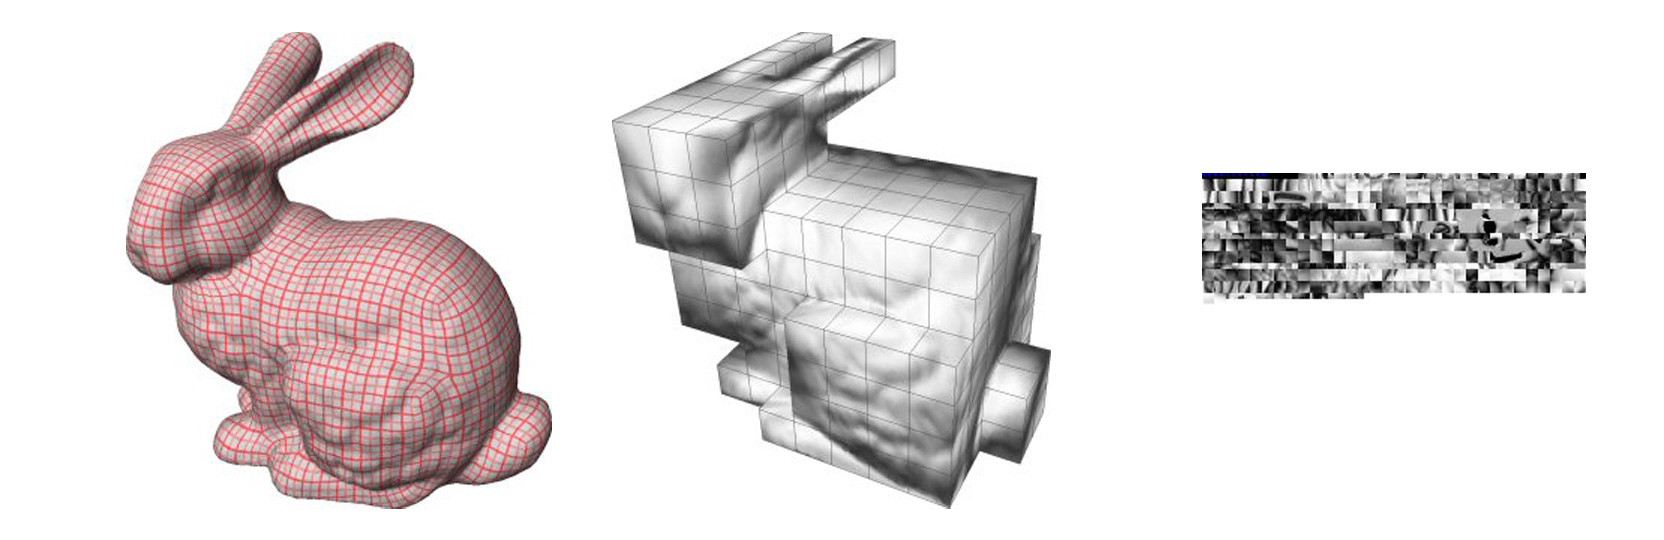
\includegraphics[width=\linewidth]{images/teaser}}

\begin{document}

\slidetitle
%\slidetableofcontents

%\slidesectionwithgraphic[bottom]{Cool Section Slide}{images/old_man}

%		\item Spielerüberforderung ...
%		 \begin{itemize}
%		 	\item durch hohe Geschwindigkeit
%		 	\item durch Perspektivenwechsel (Drehung um 90 Grad)
%		 	\item durch Gravitationsänderung
%		 \end{itemize}
%		 \item Cartoonähnliche Grafik 
%		 \item Wenige Farbtöne

%		\item Prozedurale Streckengenerierung
%		\item Beeinflussung der Streckengenerierung durch den Spieler
%		\item Hohe Geschwindigkeit
%		\item Cartoonähnliche Grafik

\slideonetoone
{Idea Development}
{
%	\begin{itemize}
%		\item Abstraktes Konzept:
%		\begin{itemize}
%			\item Start und Ziel im Raum
%			\item Schwebender Torus als Spielfigur auf der Strecke
%			\item Prozedurale Streckengenerierung durch den Spieler
%			\item Items und Powerups für Effekt
%		\end{itemize}
%		\item Wir sind die Strecke?
%		\item Wir sind das Licht?
%		\item Wir sind Licht!
%		\item Erzeugen eines Bildes
%		\item Lichtsteuerung durch Kristalle
%		\item Einfärben von Kristallen
%	\end{itemize}
	\begin{figure}
		\centering
		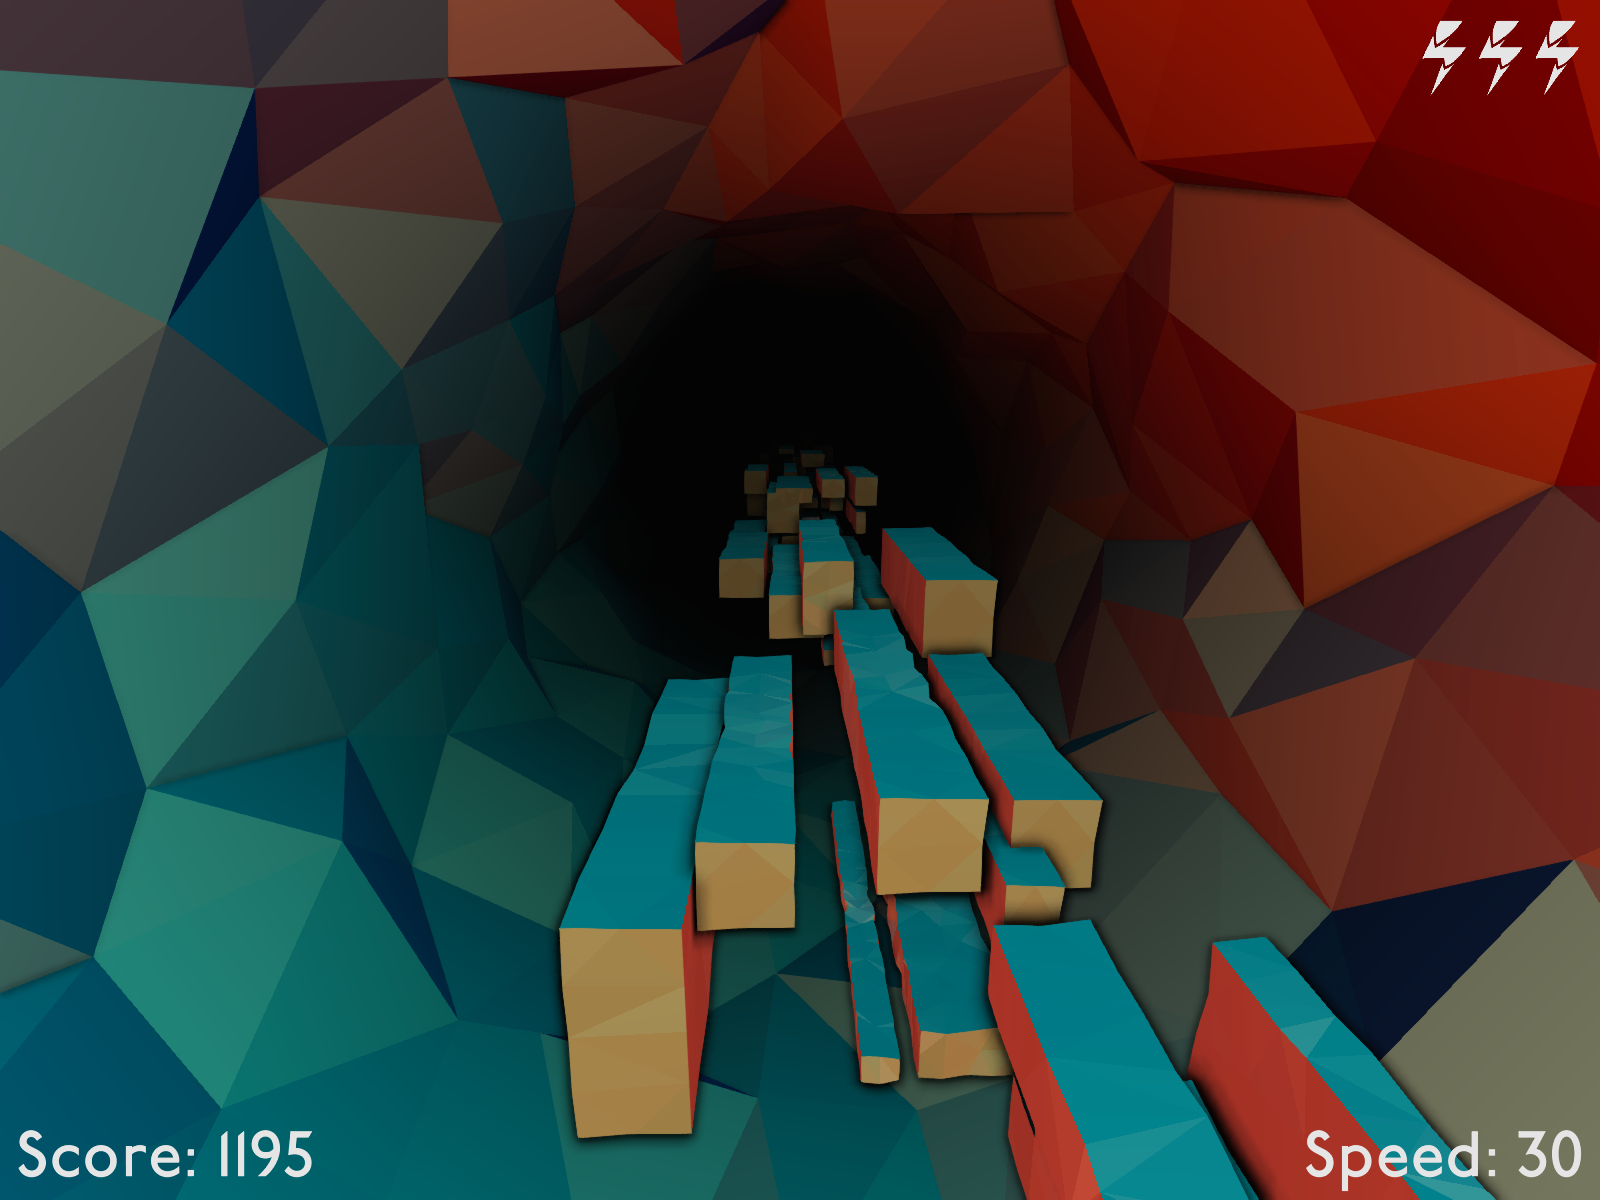
\includegraphics[width=\textwidth, height=0.7\textheight, keepaspectratio]{images/mammut_cave}
		\caption{Game Programming 2013/14: 
Mammut \linebreak A highspeed gravity racer}
		\end{figure}
}
{
	\begin{figure}
		\centering
		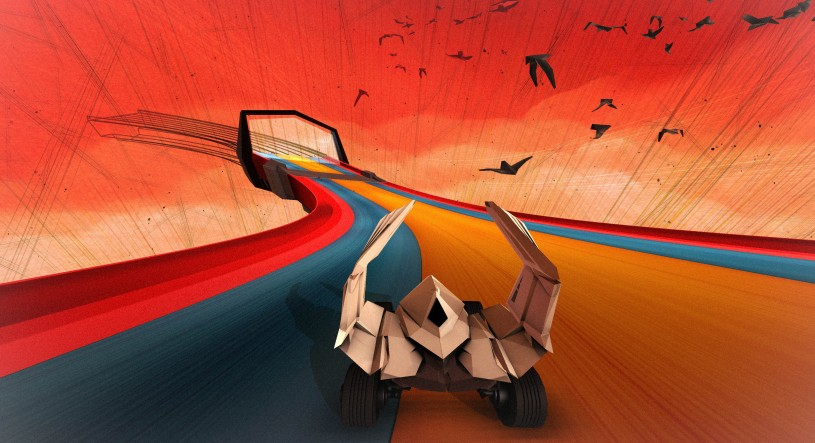
\includegraphics[width=\textwidth, height=0.7\textheight, keepaspectratio]{images/krautscape_ks1}
		\caption{Krautscape \linebreak Multiplayer racing with procedural tracks}
	\end{figure}
}

\slideonetoonetoone
{Spielprinzip}
{
	\emph{Plot}\\
	Stell dir folgende, fast alltägliche, Situation vor:\\
	Ein kleines Mädchen bewundert das für kleine Hände viel zu große Schmuckkästchen ihrer Großmutter. Es kommt, was kommen muss, und der Schmuck rutscht ihr aus der Hand. Sämtliche Kristalle fallen Richtung Boden. Und jetzt Stop. Stell dir genau diesen Moment aus der Sicht des Lichts vor. Ein Abenteuer erwartet dich.
}
{
	\pause
	\emph{Play}\\
	Der Spieler beeinflusst das Spiel, in dem er den Kristall steuert, auf den das Lichtbündel als nächstes treffen wird. Mit leichter Rotation kann man ansteuern, welcher Kristall als übernächstes vom Lichtbündel getroffen wird. Durch starke Rotation trifft man auf eine andere Oberfläche des Kristalls, und löst damit einen anderen Lichteffekt aus. Der Spieler versucht durch die Lichteffekte die Erzeugung einer ansprechenden (bunten) Kristalllandschaft zu erreichen.
}
{
	\pause
	\emph{Rules}\\
	Das Lichtbündel besitzt ein Energielevel. Er startet mit voller Energie und das Spiel ist beendet, wenn ihm die Energie ausgeht. Die Energie sinkt proportional zu der Zeit und wird von Kristallen zusätzlich beeinflusst.\\
	Sämtliche Kristalloberflächen sind mit einem bestimmten Lichteffekt verknüpft.
}

\begin{frame}{Must Have}
	\onetoone
	{
	\begin{itemize}
		\item Einfärben der Kristalle
		\item Kristalllandschaft
		\item Steuerung des nächsten Kristalls
		\item Energielevel des Lichtbündels
	\end{itemize}
	}
	{
		\begin{figure}
			\centering
			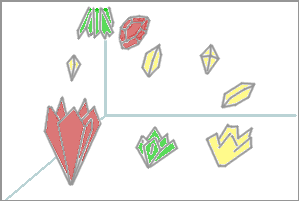
\includegraphics[width=\textwidth, height=0.4\textheight, keepaspectratio]{images/Skizzen/start-situation}
		\end{figure}
	}
	\begin{figure}
		\centering
		
\includegraphics[width=\textwidth, height=0.7\textheight, keepaspectratio]{images/chalk-154720}
	\end{figure}
\end{frame} 

\slideonetoone
{Should Have}
	{
		\begin{itemize}
			\item Abrupte Perspektivenwechsel
			\item Berechnung und Hervorhebung des übernächsten Kristalls
			\item Hindernisse
			\item Verschiedene Kristalle/Kristalleigenschaften
		\end{itemize}
		\begin{figure}
			\centering
			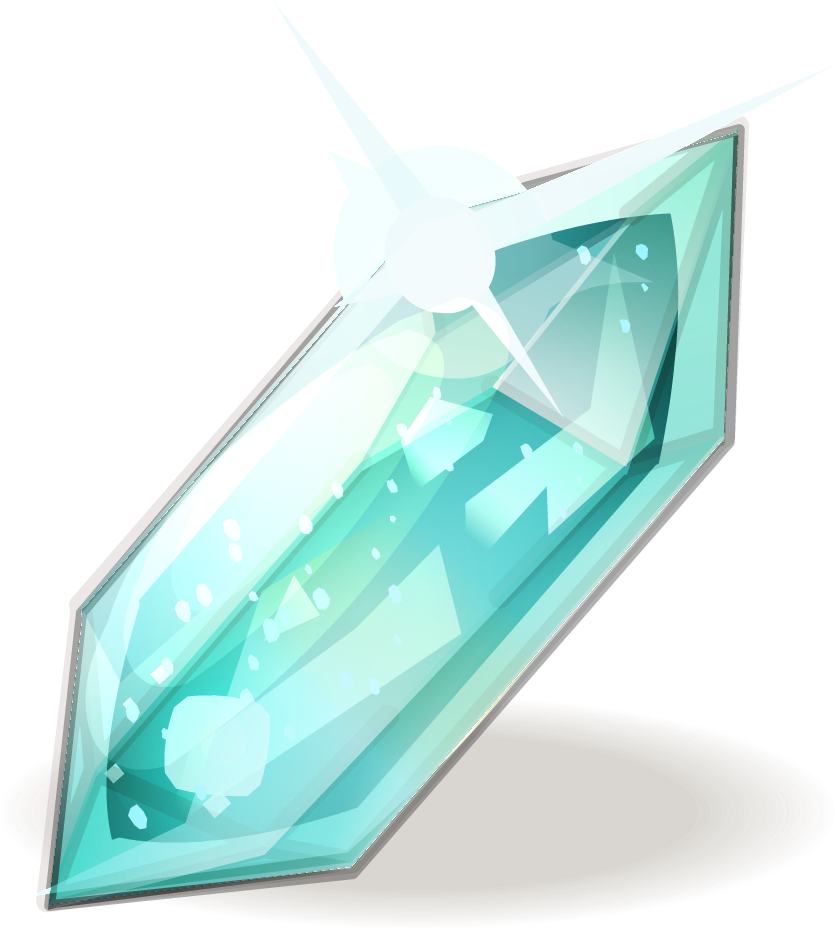
\includegraphics[width=\textwidth, height=0.35\textheight, keepaspectratio]{images/Resonanz-Kristall}
		\end{figure}
	}
	{
		\begin{figure}
			\centering
			\begin{subfigure}{\textwidth}
				\centering
				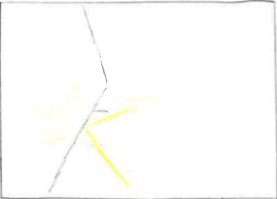
\includegraphics[width=\textwidth, height=0.35\textheight, keepaspectratio]{images/Skizzen/lichteffekt-reflektion}
			\end{subfigure}
			\begin{subfigure}{\textwidth}
				\centering
				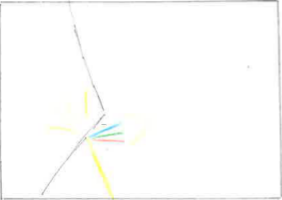
\includegraphics[width=\textwidth, height=0.35\textheight, keepaspectratio]{images/Skizzen/lichteffekt-diffus-reflektion}
			\end{subfigure}
	\end{figure}
}

\slideonetoone
{Nice to Have}
{
	\begin{itemize}
		\item Wissenschaftlichbasiertes Lichtmodell
		\item Wissenschaftlichbasiertes Farbmodell
		\item Erstellen der Kristalllandschaft durch das Herunterfallen einer Schmuckkassette
		\item Intro, bei dem man das Lichtbündel von der Sonne zur Erde verfolgt
		\item Spielende: Umwandlung der Kristalle in Würfel
	\end{itemize}
}
{
	\begin{figure}
		\centering
		\begin{subfigure}{\textwidth}
			\centering
			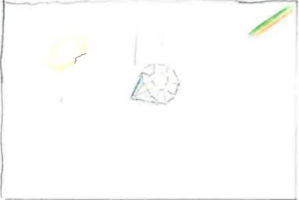
\includegraphics[width=\textwidth, height=0.35\textheight, keepaspectratio]{images/Skizzen/intro}
		\end{subfigure}
		\begin{subfigure}{\textwidth}
			\centering
			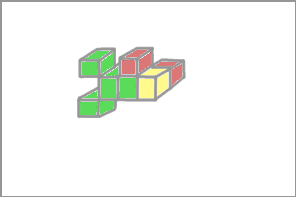
\includegraphics[width=\textwidth, height=0.35\textheight, keepaspectratio]{images/Skizzen/ende}
		\end{subfigure}
	\end{figure}
}

\begin{frame}{Meilensteine}
	\begin{itemize}
		\item \emph{Ende November}\\
		Prototyp mit Landschafts-Generierung abstrakter \glqq Kristall\grqq -Objekte im Raum. Idealerweise können wir bereits das zu steuernde Objekt ausfindig machen.
		\item \emph{Zwischenstandspräsentation}\\
		Vollständige Implementierung der Steuerung und Berechnung des übernächsten Objekts, auf das der Strahl treffen würde.
		\item \emph{Ende Januar}\\
		Kristall-Objekte werden durch real-aussehende Kristalle ersetzt und dementsprechend grafische Implementierung von Lichteffekten
		\item \emph{Anschließend}\\
		Feature-Entwicklung: Kristalleffekte, Intro, Ende
	\end{itemize}
\end{frame}
\nocite{*}
\begin{frame}[allowframebreaks]{Bibliographie}
  \bibliographystyle{apalike}
  \bibliography{../../references}
  \vfill
\end{frame}

\end{document}
